Air pollution, and it's related health impacts, is an issue that urban areas have been struggling with for many years. In Roman times the philosopher Seneca commented (after modern translation) that his disposition improved after leaving the ‘heavy air of Rome’ (\cite{seneca1969}) and after large cities in the UK started to use coal as a fuel in the 13th century, the wife of Henry VIII complained of coal smoke in the air when she visited Nottingham Castle (\cite{Brimblecombe1999}). The links between air pollution and negative effects on human health are still with us today, although the sources have changed and the visibility of the pollution has in many cases become less apparent. The Lancet's Global Burden of Disease 2013 study ranked outdoor air pollution as the  7\textsuperscript{th} highest contributing risk factor to deaths globally in 2010 (Figure \ref{fig:gbd_air_pollution}) (Lim et al (2012)).\hfill

\begin{figure}[H]
\centering
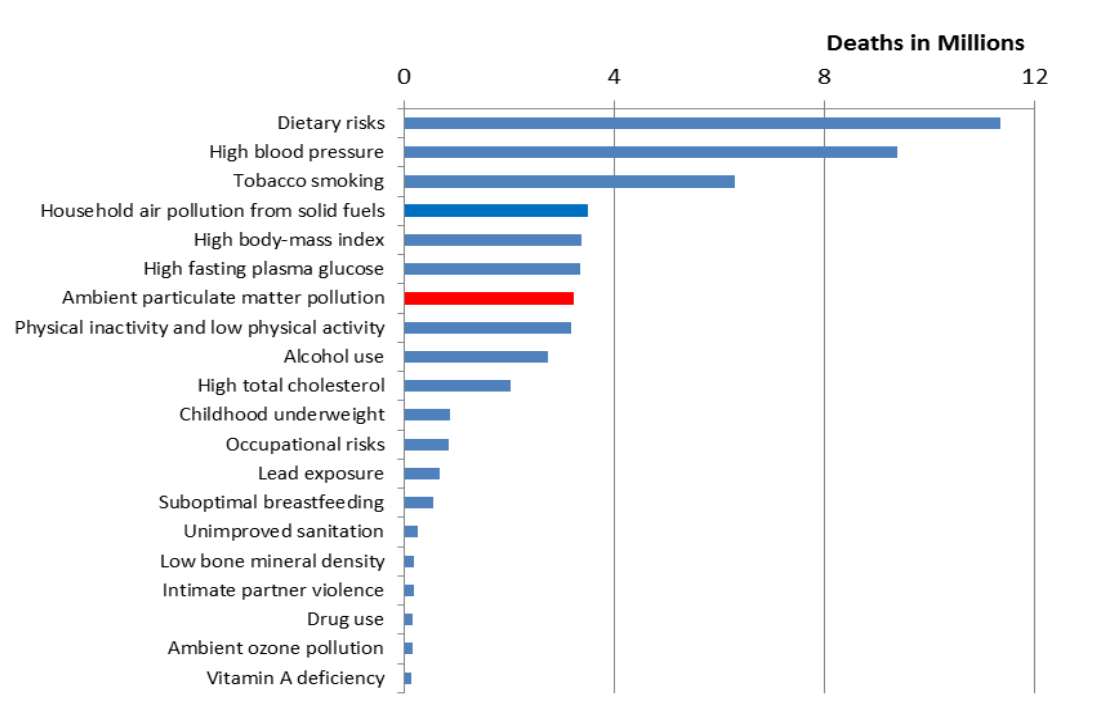
\includegraphics[scale=0.5]{gbd_air_pollution}
\caption{20 leading risk factors contributing to deaths globally in 2010}
\label{fig:gbd_air_pollution}
\end{figure}

However the methods by which exposure to air pollution is estimated are under constant revision. Due to limitations in these methods, epidemiologists may therefore be making misleading or incorrect conclusions.\hfill

This PhD begins by giving a general introduction to the subject of air pollution, it's health effects, and how health studies of air pollution have estimated population exposure in the past. It then conducts a more detailed review of dynamic exposure-health studies and the current 'state of play'. This sets the scene for novel research into the personal exposure of the population of London, and the understanding of the results thereof.\hfill